\subsection{Klirrfaktor}
Der Klirrfaktor $k=0.87$ zeigt hier das Verhältis zwischen den Amplituden der Grundschwingung und der zweiten Oberschwingung,
da nur die zweite betrachtet wird.
Entsprechend gilt dann, dass die Amplitude von $U_2$ $\qty{87}{\percent}$ von $U_1$ beträgt.

\begin{figure}
    \centering
    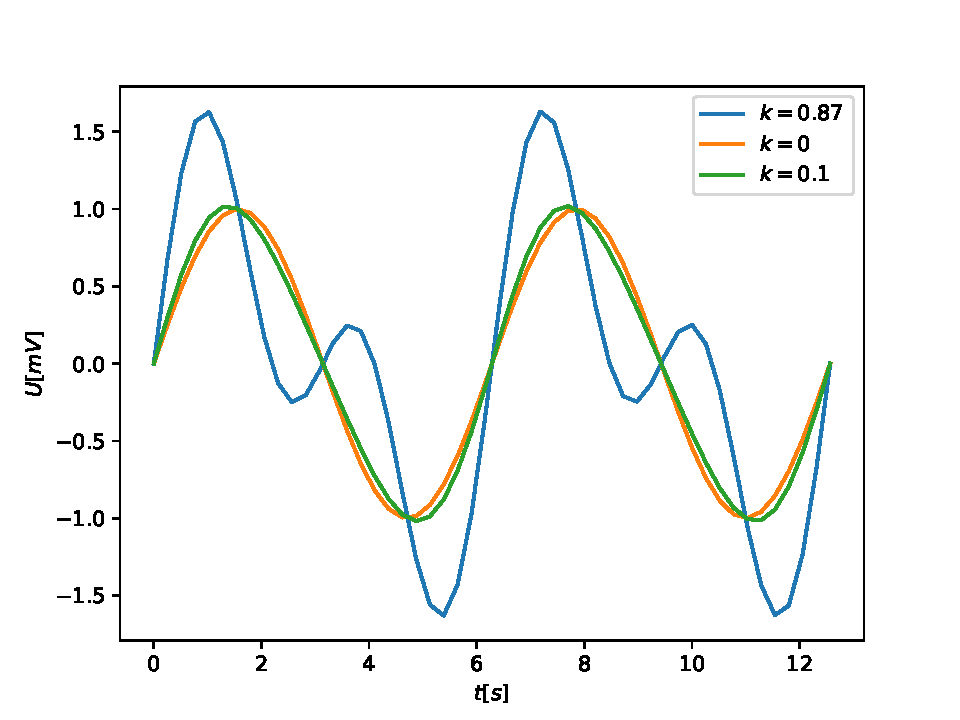
\includegraphics{./Klirr_Model.pdf}
    \caption{Modellierung von Sinusschwingungen für unterschiedliche Werte von k}
    \label{fig:klirr_mod}
\end{figure}

Wie \ref{fig:klirr_mod} modellhaft ziegt, hat ein solch großer Wert von $k$ einen signifikanten Einfluss auf den Spannungsverlauf.
Allerdings wurden für die berechnung von k störende Frequenzen höherer Ordnung vernachlässigt, was den Wert von $k$ weiter
verändern würde und die obige Beziehung zwischen $U_2$ uns $U_1$ nicht mehr gelten. Desweiteren ist es möglich, dass 
das Spannungsminimum nicht bei $\qty{150}{Hz}$ liegt, da die Frequenz nur in groben Schritten gemessen wurde verglichen mit einer
größeren Steigung in diesem Frequenzintervall, wie in \ref{fig:frequenzverhältnis} dargestellt ist. Der theoretische Wert von
$f_0$, welcher über die Eigenfrequenz über \ref{eqn:omega} berechenbar ist, beträgt $\qty{160.27(6.80)}{\hertz}$, was nahelegen würde,
dass $f_0$ größer ist, als der über \ref{frequenzen} bestimmte.